% Created 2021-09-11 Sat 08:17
% Intended LaTeX compiler: xelatex
\documentclass[letterpaper]{article}
\usepackage{graphicx}
\usepackage{grffile}
\usepackage{longtable}
\usepackage{wrapfig}
\usepackage{rotating}
\usepackage[normalem]{ulem}
\usepackage{amsmath}
\usepackage{textcomp}
\usepackage{amssymb}
\usepackage{capt-of}
\usepackage{hyperref}
\usepackage[margin=1in]{geometry}
\usepackage{fontspec}
\usepackage{indentfirst}
\setmainfont[ItalicFont = LiberationSans-Italic, BoldFont = LiberationSans-Bold, BoldItalicFont = LiberationSans-BoldItalic]{LiberationSans}
\newfontfamily\NHLight[ItalicFont = LiberationSansNarrow-Italic, BoldFont       = LiberationSansNarrow-Bold, BoldItalicFont = LiberationSansNarrow-BoldItalic]{LiberationSansNarrow}
\newcommand\textrmlf[1]{{\NHLight#1}}
\newcommand\textitlf[1]{{\NHLight\itshape#1}}
\let\textbflf\textrm
\newcommand\textulf[1]{{\NHLight\bfseries#1}}
\newcommand\textuitlf[1]{{\NHLight\bfseries\itshape#1}}
\usepackage{fancyhdr}
\pagestyle{fancy}
\usepackage{titlesec}
\usepackage{titling}
\makeatletter
\lhead{\textbf{\@title}}
\makeatother
\rhead{\textrmlf{Compiled} \today}
\lfoot{\theauthor\ \textbullet \ \textbf{2021-2022}}
\cfoot{}
\rfoot{\textrmlf{Page} \thepage}
\titleformat{\section} {\Large} {\textrmlf{\thesection} {|}} {0.3em} {\textbf}
\titleformat{\subsection} {\large} {\textrmlf{\thesubsection} {|}} {0.2em} {\textbf}
\titleformat{\subsubsection} {\large} {\textrmlf{\thesubsubsection} {|}} {0.1em} {\textbf}
\setlength{\parskip}{0.45em}
\renewcommand\maketitle{}
\author{Houjun Liu}
\date{\today}
\title{Coloumb's Law}
\hypersetup{
 pdfauthor={Houjun Liu},
 pdftitle={Coloumb's Law},
 pdfkeywords={},
 pdfsubject={},
 pdfcreator={Emacs 27.2 (Org mode 9.4.4)}, 
 pdflang={English}}
\begin{document}

\maketitle


\section{Coulomb's Law}
\label{sec:org7b329d6}
\begin{figure}[htbp]
\centering
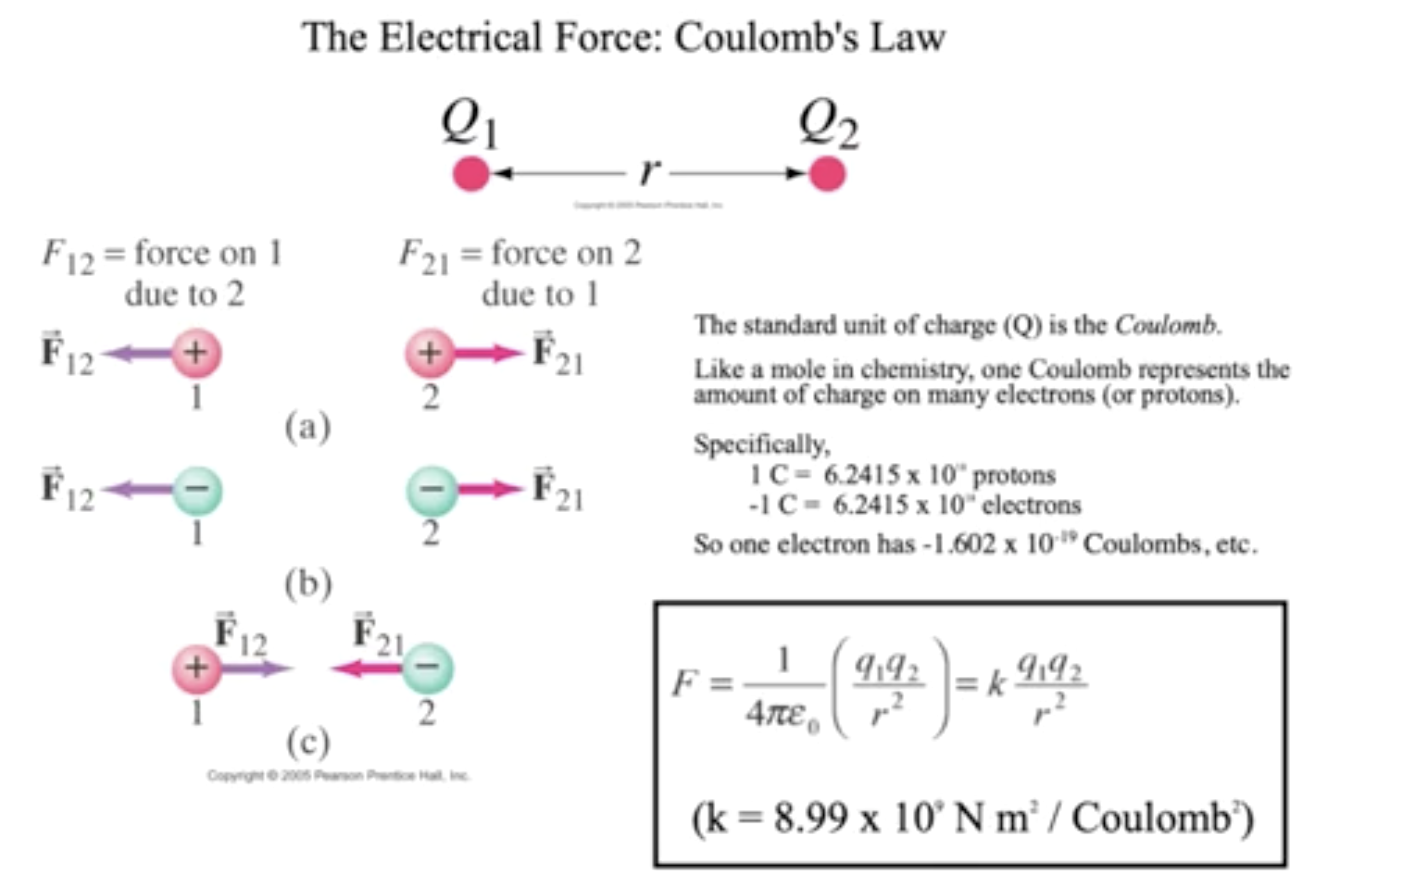
\includegraphics[width=.9\linewidth]{./Screen Shot 2020-08-24 at 7.40.48 PM.png}
\caption{Screen Shot 2020-08-24 at 7.40.48 PM.png}
\end{figure}

\begin{itemize}
\item Electrical forces gets stronger as charge increases
\item Electrical forces gets weaker as charge decreases
\end{itemize}

\begin{quote}
The magnitude of force that a particle, \(q1\), has upon another
\(q2\), is given by the Coulumb's law
\end{quote}

\definition[where $k$, a constant for change, $q_1$, change of first particle, $q_2$, change of second partical, $r^2$, distance squared]{Coulumb's Law}\{\(k\frac{q_1q_2}{r^2}\)\}
Note! The Standard Unit of Charge (Q) is the Coulomb --- a
representation for change for many electrons or many protons

\textbf{Remember this!}

\definition{Charge of an Electron}\{\(-1.602 \times 10^{-19} Q\)\}
\definition{k}\{\(8.99 \times 10^9 \frac{Nm^2}{Q^2}\)\}

\begin{quote}
E.M. forces, really, are two forces interacting with each other
\end{quote}

\textbf{Notice! Be careful with the signs when applying coulumbs law}

\begin{itemize}
\item If resulting Coulomb force > 0, force is REPULSIVE (became you
multiplied positive to positive or negative negative)
\item If resulting Coulomb force < 0, force is ATTRACTIVE (became you
multiplied positive to negative)
\end{itemize}

Coloumb's law could be applied when modeling
\href{KBhPHYS201ElectricFields.org}{KBhPHYS201ElectricFields} Electric
fields to see how particles interact and how they influence each other.

\subsection{Guided Problem Solve}
\label{sec:org717f94f}
Special care must be taken for solving these problems w.r.t. to both
vector direction and multiple-atom-interactions
\href{KBhPHYS201GuidedProblemCoulomb.org}{KBhPHYS201GuidedProblemCoulomb}

\subsection{Here's something! DNA Replication}
\label{sec:org3b03329}
\begin{figure}[htbp]
\centering
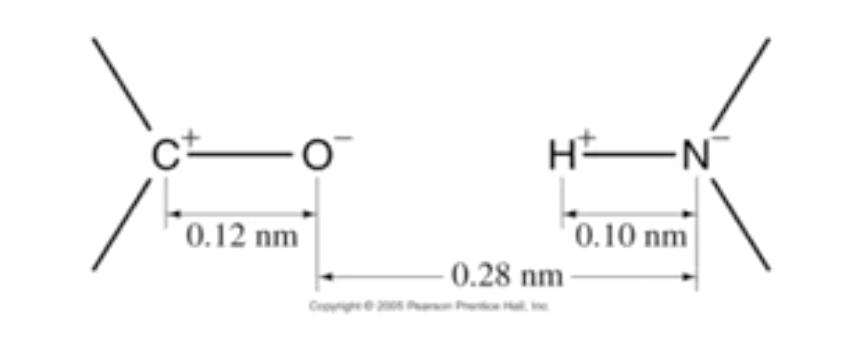
\includegraphics[width=.9\linewidth]{./Screen Shot 2020-08-24 at 8.20.15 PM.png}
\caption{Screen Shot 2020-08-24 at 8.20.15 PM.png}
\end{figure}

The question is\ldots{} Between these four atoms, \emph{how many do we need to
calculate to find if these two repel or attract?}

This is fairly simple. Because of the fact every force between each pair
of atoms between these two elements needs to be calculated. So\ldots{} 2 (on
the left) times 2 (on the right) = 4.

If these repel, the don't combine. If they attract, of course they do.
\end{document}
